\section{Construction}
In order to complete the construction, it is necessary to define the addition, multiplication, negation and inversion of constructable numbers.
The following chapter presents a proof schema, whereby lines and circles are used to demonstrate that the desired point is contained within their intersection. As the proofs are lengthy and repetitive, they have been omitted from the handout. Instead, the construction and underlying concepts are presented.
The complete proofs can be found in the blueprint.

\begin{lemma}[Addition of complex numbers]
    \label{lem:construction_add}
    For $z_1, z_2 \in M_{\infty}$ is $z_1 + z_2 \in M_{\infty}$.
\end{lemma}
This construction is taken from \cite{JAN_SCHROEER:2023}.\\
One can construct the point $z_1 + z_2$ by drawing a circle with center $z_1$ and radius $\|z_2\|$ and a circle with center $z_2$ and radius $\|z_1\|$ and taking the intersection of the two circles Fig.\ref{Fig.2}.

\begin{figure}[h!]
    \centering
    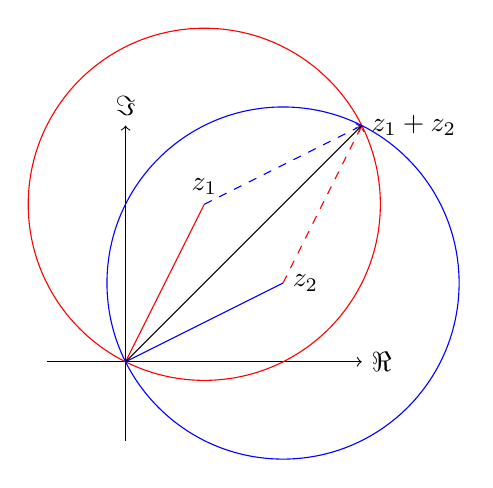
\begin{tikzpicture}
        \draw[->] (-1,0) -- (3,0) node[right] {$\Re$};
        \draw[->] (0,-1) -- (0,3) node[above] {$\Im$};
        \draw (0,0) -- (1,2) node[above] {$z_1$}[red];
        \draw (0,0) -- (2,1) node[right] {$z_2$}[blue];
        \draw (1,2) circle (2.2360679775)[red];
        \draw (2,1) circle (2.2360679775)[blue];
        \draw[dashed,->] (1,2) -- (3,3)[blue];
        \draw[dashed,->] (2,1) -- (3,3)[red];
        \draw (0,0) -- (3,3) node[right] {$z_1 + z_2$};
    \end{tikzpicture}
    \caption{Construction of $z_1 + z_2$}
    \label{Fig.2}
\end{figure}

\begin{lstlisting}
lemma add_M_Inf (M: Set ℂ) (h₀: (0:ℂ)∈ M) (z₁ z₂ : ℂ) (hz₁ : z₁ ∈ (M_inf M)) (hz₂ : z₂ ∈ (M_inf M)):
        z₁ + z₂ ∈ (M_inf M) := by
    let c₁ : Construction.circle := {c := z₁, r := (dist 0 z₂)}
    let c₂ : Construction.circle := {c := z₂, r := (dist 0 z₁)}
    let l: line := {z₁ := z₁, z₂ := 0}
    have hc₁ : c₁ ∈ C (M_inf M) := by
    refine ⟨z₁, 0, z₂, ?_, hz₁,M_M_inf M h₀, hz₂⟩
    simp [c₁]
    have hc₂ : c₂ ∈ C (M_inf M) := by
    refine ⟨z₂, 0, z₁, ?_,hz₂,M_M_inf M h₀,hz₁⟩
    simp [c₂]
    by_cases h: (z₁ = z₂)
    . by_cases hz₁0: (z₁ = 0)
    . simp only [hz₁0, zero_add, hz₂]
    . have hl : l ∈ L (M_inf M) := by
        refine ⟨z₁, 0, ?_, hz₁, M_M_inf M h₀, hz₁0⟩
        simp [l, hz₁0]
        apply ilc_M_inf M
        refine ⟨c₁, hc₁, l, hl, ⟨?_, ⟨2,?_⟩⟩⟩
        . simp [circle.points, h]
        . simp [h, two_mul]
    refine icc_M_inf M ⟨c₁,hc₁, c₂,hc₂, ?_⟩
    simp [circle.points, Set.mem_inter_iff]
    exact circle_not_eq_iff  (by exact h)
\end{lstlisting}

\begin{lemma}[Negative complex numbers]
    \label{lem:construction_neg}
    \lean{z_neg_M_inf}
    \leanok
    \uses{def:set_of_constructable_points}
    For $z \in M_{\infty}$,  $-z$ is in $M_{\infty}$.
\end{lemma}
This construction is taken from \cite{JAN_SCHROEER:2023}.\\
To get the point $-z$ we can use the second intersection of the line through $0$ and $z$ with circle with center $0$ and radius $\|z\|$ Fig.\ref{Fig.1}.

\begin{figure}[h!]
    \centering
    \begin{tikzpicture}
        \draw[->] (-1,0) -- (3.5,0) node[right] {$\Re$};
        \draw[->] (0,-1) -- (0,3.5) node[above] {$\Im$};
        \coordinate[label=45:$z$] (z) at (2,2);
        \coordinate[label=-135:$-z$] (zminus) at (-2,-2);
        \draw (zminus) -- (z) [blue];
        \draw (0,0) circle (2.82)[red];
        \fill[black] (z) circle (2pt);
        \fill[black] (zminus) circle (2pt);
    \end{tikzpicture}
    \caption{Construction of $-z$}
    \label{Fig.1}
\end{figure}

\begin{lstlisting}
lemma z_neg_M_inf (M: Set ℂ) (h₀: (0:ℂ)∈ M) (z : ℂ) 
        (hz : z ∈ (M_inf M)) : -z ∈ (M_inf M) := by
    by_cases z0:(z=0)
    . simp [z0, M_M_inf M h₀]
    let l : line := {z₁ := 0, z₂ := z}
    let c : Construction.circle := {c := 0, r := (dist 0 z)}
    have hl : l ∈ L (M_inf M) := by
      refine ⟨0, z, ?_, M_M_inf M h₀, hz, ?_⟩
      simp only [l]
      simp  [eq_comm, z0]
    have hc : c ∈ C (M_inf M) := by
      refine ⟨0, 0, z, ?_, M_M_inf M h₀, M_M_inf M h₀, hz⟩
      simp [l, c]
    apply ilc_M_inf M
    refine ⟨c , hc, l, hl, ?_⟩
    simp [circle.points, line.points]
    refine ⟨2, (by push_cast; ring_nf)⟩
\end{lstlisting}

\begin{lemma}[Multiplication of positive real numbers]
    \label{lem:construction_mul}
    \lean{ab_in_M_inf}
    \leanok
    \uses{def:set_of_constructable_points}
    For $a, b \in M_{\infty}\cap\R$, $a \cdot b \in M_{\infty}$.
\end{lemma}
This construction is taken from \cite{cox2012galois}.\\
To get the point $a\cdot b$ we draw a line through $a$ and $\imath$ and a parallel line through $\imath b$. The intersection of the second line with the real axis is $a\cdot b$ Fig.\ref{Fig.5}.

\begin{figure}[h!]
    \centering
    \begin{tikzpicture}
        \draw[->] (-0.5,0) -- (5,0) node[right] {$\Re$};
        \draw[->] (0,-0.5) -- (0,3) node[above] {$\Im$};
        \coordinate[label=135:$\imath$] (i) at (0,1);
        \coordinate[label=-90:$a$] (a) at (2,0);
        \coordinate[label=135:$\imath b$] (ib) at (0,2);
        \coordinate[label=-90:$ab$] (ab) at (4,0);
        \fill[black] (i) circle (2pt);
        \fill[black] (a) circle (2pt);
        \fill[black] (ib) circle (2pt);
        \fill[black] (ab) circle (2pt);
        \draw (a) -- (i);
        \draw (ib) -- (ab);
    \end{tikzpicture}
    \caption{Construction of $z_1 \cdot z_2$}
    \label{Fig.5}
\end{figure}

\begin{remark}
    If you look at how you chose the representatives of the parallel line $x = a+In-b$ and $y=Ib$, you can prove that they are in $M_{\infty}$ without the first line, so you can prove this with only two lines.
\end{remark}

\begin{lstlisting}
lemma ab_in_M_inf (M: Set ℂ) (h₀: 0 ∈ M) (h₁: 1 ∈ M) (a b :ℝ) 
    (ha: ↑a ∈ M_inf M) (hb: ↑b ∈ M_inf M): ↑(a * b) ∈ M_inf M := by
  by_cases h: a*b = 0
  . rw[h]
    exact M_M_inf M h₀
  let l : line := {z₁ := a+I*b-I, z₂ := I*b}
  let lr : line := {z₁ := 1, z₂ := 0}
  have hl : l ∈ L (M_inf M) := by
    refine ⟨(a+I*b-I), I*b, (by simp), ?_, ir_M_inf _ h₀ h₁ _ hb, ?_⟩
    . simp only [sub_M_Inf, add_M_Inf, ir_M_inf M h₀ h₁ b hb, imath_M_inf, h₀, h₁, ha]
    simp [ext_iff]
  have hlr : lr ∈ L (M_inf M) := by
    refine ⟨1, 0, (by simp only), M_M_inf M h₁,  M_M_inf M h₀, ?_⟩
    simp only [ne_eq, one_ne_zero, not_false_eq_true]
  refine ill_M_inf M ⟨l,hl, lr, hlr, ⟨⟨b, ?_⟩, ⟨a*b, ?_⟩⟩, ?_ ⟩
  push_cast; ring_nf
  push_cast; ring_nf
  refine line_not_eq_if'  l lr ⟨0, ⟨?_, ?_⟩⟩
  . simp[line.points]
  . simp[line.points, ext_iff, sub_mul, mul_sub, sub_eq_zero]
    rw[mul_eq_zero, or_comm, Mathlib.Tactic.PushNeg.not_or_eq] at h
    exact h
\end{lstlisting}

\begin{corollary}[Multiplication of complex numbers]
    \label{cor:construction_mul_complex}
    %\lean{mul_in_M_inf}
    %\leanok
    \uses{def:set_of_constructable_points}
    For $z_1, z_2 \in M_{\infty}$ is $z_1 \cdot z_2$ in $M_{\infty}$.
\end{corollary}
\begin{proof}
    \uses{lem:construction_mul, lem:construction_add, cor:construction_sub, lem:construction_real, lem:construction_imag}
    Let $z_1 = a + \imath b$ and $z_2 = c + \imath d$. Then $$z_1 \cdot z_2 = (a + \imath b) \cdot (c + \imath d) = (a \cdot c - b \cdot d) + \imath (a \cdot d + b \cdot c).$$
    By combining the Lemmas \ref{lem:construction_add}, \ref{lem:construction_mul} with subtraction, real and imaginary part we get that $z_1 \cdot z_2 \in M_{\infty}$.
\end{proof}

\begin{lstlisting}
lemma z_iff_re_im_M_inf (M: Set ℂ) (h₀: 0 ∈ M) (h₁: 1 ∈ M) (z: ℂ): 
    z ∈ M_inf M ↔ ↑z.re ∈ M_inf M ∧ ↑z.im ∈ M_inf M := sorry

lemma mul_M_inf (M: Set ℂ) (h₀: 0 ∈ M) (h₁: 1 ∈ M) (a b :ℂ ) 
    (ha: a ∈ M_inf M) (hb: b ∈ M_inf M): a * b ∈ M_inf M:= by
  refine (z_iff_re_im_M_inf M h₀ h₁ (a * b)).mpr ⟨?_, ?_⟩ <;>
  simp only [mul_re, mul_im, ofReal_sub, ofReal_add]
  . apply sub_M_Inf M h₀
    exact ab_in_M_inf M h₀ h₁ _ _ (real_in_M_inf M h₀ h₁ a ha) 
        (real_in_M_inf M h₀ h₁ b hb)
    exact ab_in_M_inf M h₀ h₁ _ _ (im_in_M_inf M h₀ h₁ a ha) 
        (im_in_M_inf M h₀ h₁ b hb)
  . apply add_M_Inf M h₀
    exact ab_in_M_inf M h₀ h₁ _ _ (real_in_M_inf M h₀ h₁ a ha) 
        (im_in_M_inf M h₀ h₁ b hb)
    exact ab_in_M_inf M h₀ h₁ _ _ (im_in_M_inf M h₀ h₁ a ha)
        (real_in_M_inf M h₀ h₁ b hb)
\end{lstlisting}

\begin{lemma}[Inverse of a pos real number]
    \label{lem:construction_inv}
    \lean{ainv_in_M_inf}
    \leanok
    \uses{def:set_of_constructable_points}
    If $a \in M_{\infty}\cap\R$, then $a^{-1}$ is in  $M_{\infty}$.
\end{lemma}

This can be constructed analog to the multiplication of positive real numbers. Using the fact that $a\cdot a^{-1} = 1$. Draw a line through $1$ and $\imath a$ and a parallel line through $\imath$. The intersection of the second line with the real axis is $a^{-1}$ Fig.\ref{Fig.6}.
\begin{proof}
    \uses{def:line, def:set_of_lines, lem:ill_M_inf, lem:construction_imath_r, cor:construction_imath, lem:construction_add, cor:construction_sub}
    Without loss of generality we can assume that $a \ne 0$.\\
    Then the proof is analog to the proof of Lemma \ref{lem:construction_mul}, we just need two lines $l = \{1-\imath a + \imath, \imath\}$ and $l_{\Re} = \{1,0\}$.\\
    That there are in $\mathcal{L(M_{\infty})}$ follows analog to the proof of Lemma \ref{lem:construction_mul}.\\ 
    So we have just to show that $a^{-1} \in l$, i.e. $\exists t: t  (1 - \imath a + \imath) + (1 - t)  I = a^{-1}$ $$t  (1 - \imath a + \imath) + (1 - t)  \imath \stackrel{t:=a^{-1}}{=}  a^{-1} - a^{-1} \imath a + a^{-1}\imath + \imath - a^{-1}\imath = a^{-1}.$$
    The rest follws analog.
\end{proof}
\begin{figure}[h!]
    \centering
    \begin{tikzpicture}
        \draw[->] (-1,0) -- (2,0) node[right] {$\Re$};
        \draw[->] (0,-1) -- (0,3) node[above] {$\Im$};
        \coordinate[label=135:$\imath$] (i) at (0,1);
        \coordinate[label=-90:$1$] (1) at (1,0);
        \coordinate[label=135:$\imath a$] (ia) at (0,2);
        \coordinate[label=-90:$a^{-1}$] (ainv) at (0.5,0);
        \fill[black] (i) circle (2pt);
        \fill[black] (1) circle (2pt);
        \fill[black] (ia) circle (2pt);
        \fill[black] (ainv) circle (2pt);
        \draw (1) -- (ia);
        \draw (i) -- (ainv);
    \end{tikzpicture}
    \caption{Construction of $z^{-1}$}
    \label{Fig.6}
\end{figure}

\begin{lstlisting}
lemma ainv_in_M_inf (M: Set ℂ) (h₀: 0 ∈ M) (h₁: 1 ∈ M) (a :ℝ) 
        (ha: ↑a ∈ M_inf M): ↑(a⁻¹) ∈ M_inf M := by
    by_cases h: a = 0
    . simp [h]
      exact M_M_inf _ h₀
    let l: line := {z₁ := 1-I*a+I, z₂ := I}
    let lr : line := {z₁ := 1, z₂ := 0}
    have hl : l ∈ L (M_inf M) := by
      refine ⟨(1-I*a+I), I, (by simp), ?_, imath_M_inf M h₀ h₁, ?_⟩
      . apply add_M_Inf M h₀ (1-I*a) I ?_ (imath_M_inf M h₀ h₁)
        exact sub_M_Inf M h₀ 1 (I*a) (M_M_inf M h₁) 
            (mul_M_inf M h₀ h₁ _ _ (imath_M_inf M h₀ h₁) ha)
      simp [ext_iff]
    have hlr : lr ∈ L (M_inf M) := by
      refine ⟨1, 0, (by simp), M_M_inf M h₁, M_M_inf M h₀, ?_⟩
      simp
    refine ill_M_inf M ⟨l, hl, lr, hlr, ⟨⟨a⁻¹, ?_⟩ , ⟨a⁻¹, ?_⟩⟩, ?_⟩
    . ring_nf
    simp [h, mul_rotate]
    . simp only [ofReal_inv, mul_one, mul_zero, add_zero]
    refine line_not_eq_if' l lr ⟨0, ⟨?_, ?_⟩⟩
    . simp [line.points]
    . simp [line.points, ext_iff]
\end{lstlisting}
\begin{remark}
    The non-terminal \verb|simp| and the rest without \verb|only| are only used for better readability.
\end{remark}

\begin{corollary}[Inverse of a complex number]
    \label{cor:inv_M_inf}
    \lean{inv_M_inf, z_inv_eq}
    \leanok
    \uses{def:set_of_constructable_points}
    If $z \in M_{\infty}$, then $z^{-1}$ is in  $M_{\infty}$.
\end{corollary}
\begin{proof}
    \uses{lem:construction_inv, lem:construction_mul, cor:construction_sub, lem:construction_real, lem:construction_imag, lem:construction_add}
    For $z \in M_{\infty}$ we can write $z = a + \imath b$ with $a, b \in \R$. Then
    $$z^{-1} = \frac{1}{z} = \frac{\overline{z}}{z\overline{z}} = \frac{a - \imath b}{a^2+b^2}= (a - \imath b) \cdot (aa+bb)^{-1}.$$
    Now we can again combine the lemmas for addition \ref{lem:construction_add}, subtraction [blue print], multiplication \ref{cor:construction_mul_complex} and the corollary for the inverse of a positive real number \ref{lem:construction_inv} with the exists of real an imaginary [blue print] part to conclude that $z^{-1} \in M_{\infty}$.
\end{proof}
\begin{lstlisting}
lemma z_inv_eq (z:ℂ) (hz: z ≠ 0): z⁻¹ = z.re / (z.re^2+z.im^2)-(z.im/ (z.re^2+z.im^2) )*I := sorry

lemma inv_M_inf (M: Set ℂ) (h₀: 0 ∈ M) (h₁: 1 ∈ M) (a :ℂ ) 
        (ha: a ∈ M_inf M): a⁻¹ ∈ M_inf M:= by
    by_cases h: a = 0
    . simp only [h, inv_zero]
    exact M_M_inf _ h₀
    simp_rw [z_inv_eq _ h, Field.div_eq_mul_inv, pow_two]
    apply sub_M_Inf M h₀
    . apply mul_M_inf M h₀ h₁ _ _ (real_in_M_inf M h₀ h₁ a ha)
    norm_cast
    apply ainv_in_M_inf M h₀ h₁
    push_cast
    apply add_M_Inf M h₀
    exact mul_M_inf M h₀ h₁ _ _ (real_in_M_inf M h₀ h₁ _ ha) 
        (real_in_M_inf M h₀ h₁ _ ha)
    exact mul_M_inf M h₀ h₁ _ _ (im_in_M_inf M h₀ h₁ _ ha) 
        (im_in_M_inf M h₀ h₁ _ ha)
    . apply mul_M_inf M h₀ h₁ _ _ ?_ (imath_M_inf M h₀ h₁)
    apply mul_M_inf M h₀ h₁ _ _ (im_in_M_inf M h₀ h₁ _ ha)
    norm_cast
    apply ainv_in_M_inf M h₀ h₁
    push_cast
    apply add_M_Inf M h₀
    exact mul_M_inf M h₀ h₁ _ _ (real_in_M_inf M h₀ h₁ _ ha) 
        (real_in_M_inf M h₀ h₁ _ ha)
    exact mul_M_inf M h₀ h₁ _ _ (im_in_M_inf M h₀ h₁ _ ha) 
        (im_in_M_inf M h₀ h₁ _ ha)
\end{lstlisting}
\newpage